% !Mode:: "TeX:UTF-8"
\chapter{luaVM的web移植}

\section{lua简介}

Lua是一个小巧的脚本语言。由巴西里约热内卢天主教大学
(Pontifical Catholic University of Rio de Janeiro)里的一个研究小组,
由Roberto Ierusalimschy、Waldemar Celes 和 Luiz Henrique de Figueiredo所组成并于1993年开发。 
Lua语言开发之初的目的,并不是编写一个强大的编程语言,正相反,Roberto希望的是开发一个小巧灵活、平台无关的编程语言,作为C/C++的补充,为C++提供脚本化和热更新支持 (因为那个时候C编译器编译速度并不理想),借助脚本化和热更新的特效,Lua可以为应用程序提供灵活的扩展和定制功能,也是因为Roberto并没有把Lua设计为独立的编程语言,Lua并没有提供强大的标准库,而是内置了少量但够用内置函数,没有强大的库限制了Lua不适合作为独立开发应用程序的语言\footnote{有了luaDist和luaRocks之后情况大为改观}。

Lua 还有一个和Lua主干项目同时进行开发的高速Lua虚拟机项目,名为LuaJIT,提供在特定体系结构和操作系统上的的JIT功能,可以显著加速Lua代码运行的速度。

Lua完全由POSIX C写成,没有任何外部依赖,在任何支持C语言的操作系统和硬件上 (几乎所有的平台)都可以编译运行。一个完整的 Lua 虚拟机/解释器出容量不超过200kb,Lua虚拟机的性能也很好,在众多脚本语言解释器中,Lua解释器仅仅慢于JavaScript解释器 (在谷歌的JavaScript解释器V8出现以前,Lua解释器就是最快的)。

Lua虚拟机完全由C语言写成,因此可以很容易的包含在 C/C++ 代码中。因为最后的二进制文件包含了完整的 Lua 虚拟机,可以在 C/C++ 代码中很轻松的调用 lua 的各种方法。但是,除此之外,Lua 还能调用 C/C++ 的方法\footnote{通过回调},这个特性极大的增加了 Lua 的使用范围和使用场景。不单单能够作为应用程序的扩展脚本文件,还能用来当做说明文件,比如Rockstar的RAGE引擎,网易的《大话西游》系列游戏,还有动视暴雪的《魔兽世界》游戏,就使用 Lua 文件作为配置描述文件,代替了常见的配置文件,比如XML文件、ini文件等。使用XML或者ini文件,运行时需要文本解析,而Lua代码直接运行,使用Lua脚本作为配置文件,性能也更好一些。

这一切都决定了Lua是作为嵌入式脚本的最佳选择\upcite{ierusalimschy1996lua}。

\section{lua virtual machine的特征}

Lua 虚拟机在传统 C++游戏开发中,一般当作一个黑箱运行,
我们只给他一个输入,然后获取他的输出,lua虚拟机,几乎不对外暴露接口。
这种情况下,lua虚拟机就是一个相对独立的系统。

也就是说,lua virtual machine 相当于一个“黑箱程序”。

\section{“黑箱程序”释义}

黑箱亦称"黑盒"或"黑匣"。它指在各种主观条件和客观条件的限制下,无法搞清楚其中的内部构造方法。只能通过在外部,进行各种观测和实验,来研究其中的各种特性以及功能的系统。例如计算机的显卡、锁上引擎盖的汽车、关闭了配置室的程序机房一样,都能够将之当做为一个是“黑盒”。我们把外部对黑箱的各种作用行为称为黑箱的输入,而把黑箱对各种外部作用而产生的反应行为称为黑箱的输出。

黑箱方法,又称"黑箱系统辨识法"。是指通过对外部输入的黑盒信息和黑盒输出信息的观测,探索了黑盒结构和内部机制的方法。“黑盒”是指对事物的内部结构和机制的直接观察不可。要注意黑盒的整体功能和方法,并且具有抽象方法和模型方法的特点。

所谓的“黑盒”方法是通过对输入、输出和动态过程的系统调查,而不是通过直接研究其内部结构,定量或定性地了解系统的各种作用、功能以及行为特点,并探讨一种控制方法的内在结构和机理。

黑盒法是在黑盒子里没有打开,只是通过外部观察、实验,找出了输入与输出的关系,从而对黑盒的功能和特点,使用一种科学的方法对其结构和机理进行探索。


\section{最简单的“黑箱程序”实例}

其实最简单的“黑箱程序”,就是hello world程序,只不过用C语言编写。
我们希望用C语言编写的hello world程序能在浏览器中正确的运行,表现出Web程序应有的效果。
我这个称这个程序是黑箱程序,因为我们只关心C代码在浏览器中运行的最终结果,并不关心生成JavaScript代码的容量、暴露接口数、实际执行过程等细节问题。

\section{lua virtual machine 移植过程}

移植lua virtual machine的过程比较简单。

\subsection{lua移植过程}

lua移植过程入下所述:

\begin{enumerate}[itemindent=2em]
    \item 下载lua源代码,我使用的是lua 5.2.4版本;
    \item 在lua源代码目录下执行\ref{bash-luavm}命令;
        \begin{lstlisting}[
    		language={bash},
    		caption={lua程序的源代码编译命令},
    		label={bash-luavm},
		]

		make emscripten
		\end{lstlisting}
	\item 得到lua.vm.js文件。
\end{enumerate}

{\heiti 解释 : } make emscripten是emscripten工具集给的一个简易扩展命令,可以告诉make工具,
使用emcc代替makefile中定义的C/C++编译器

\subsection{lua交互式解释器代码}

附录\ref{html-lua-repl}所示代码是lua在线REPL(Read eval print loop)的关键代码,其中,CodeMirror是我引用的一个第三方库,作用是代码高亮。

\subsection{lua交互式解释器运行效果}

图\ref{lua-vm-repl}展示了lua REPL在浏览器中运行的效果。

\begin{figure}[h!] % [h!] 表示尽量排在当前位置
    \centering
    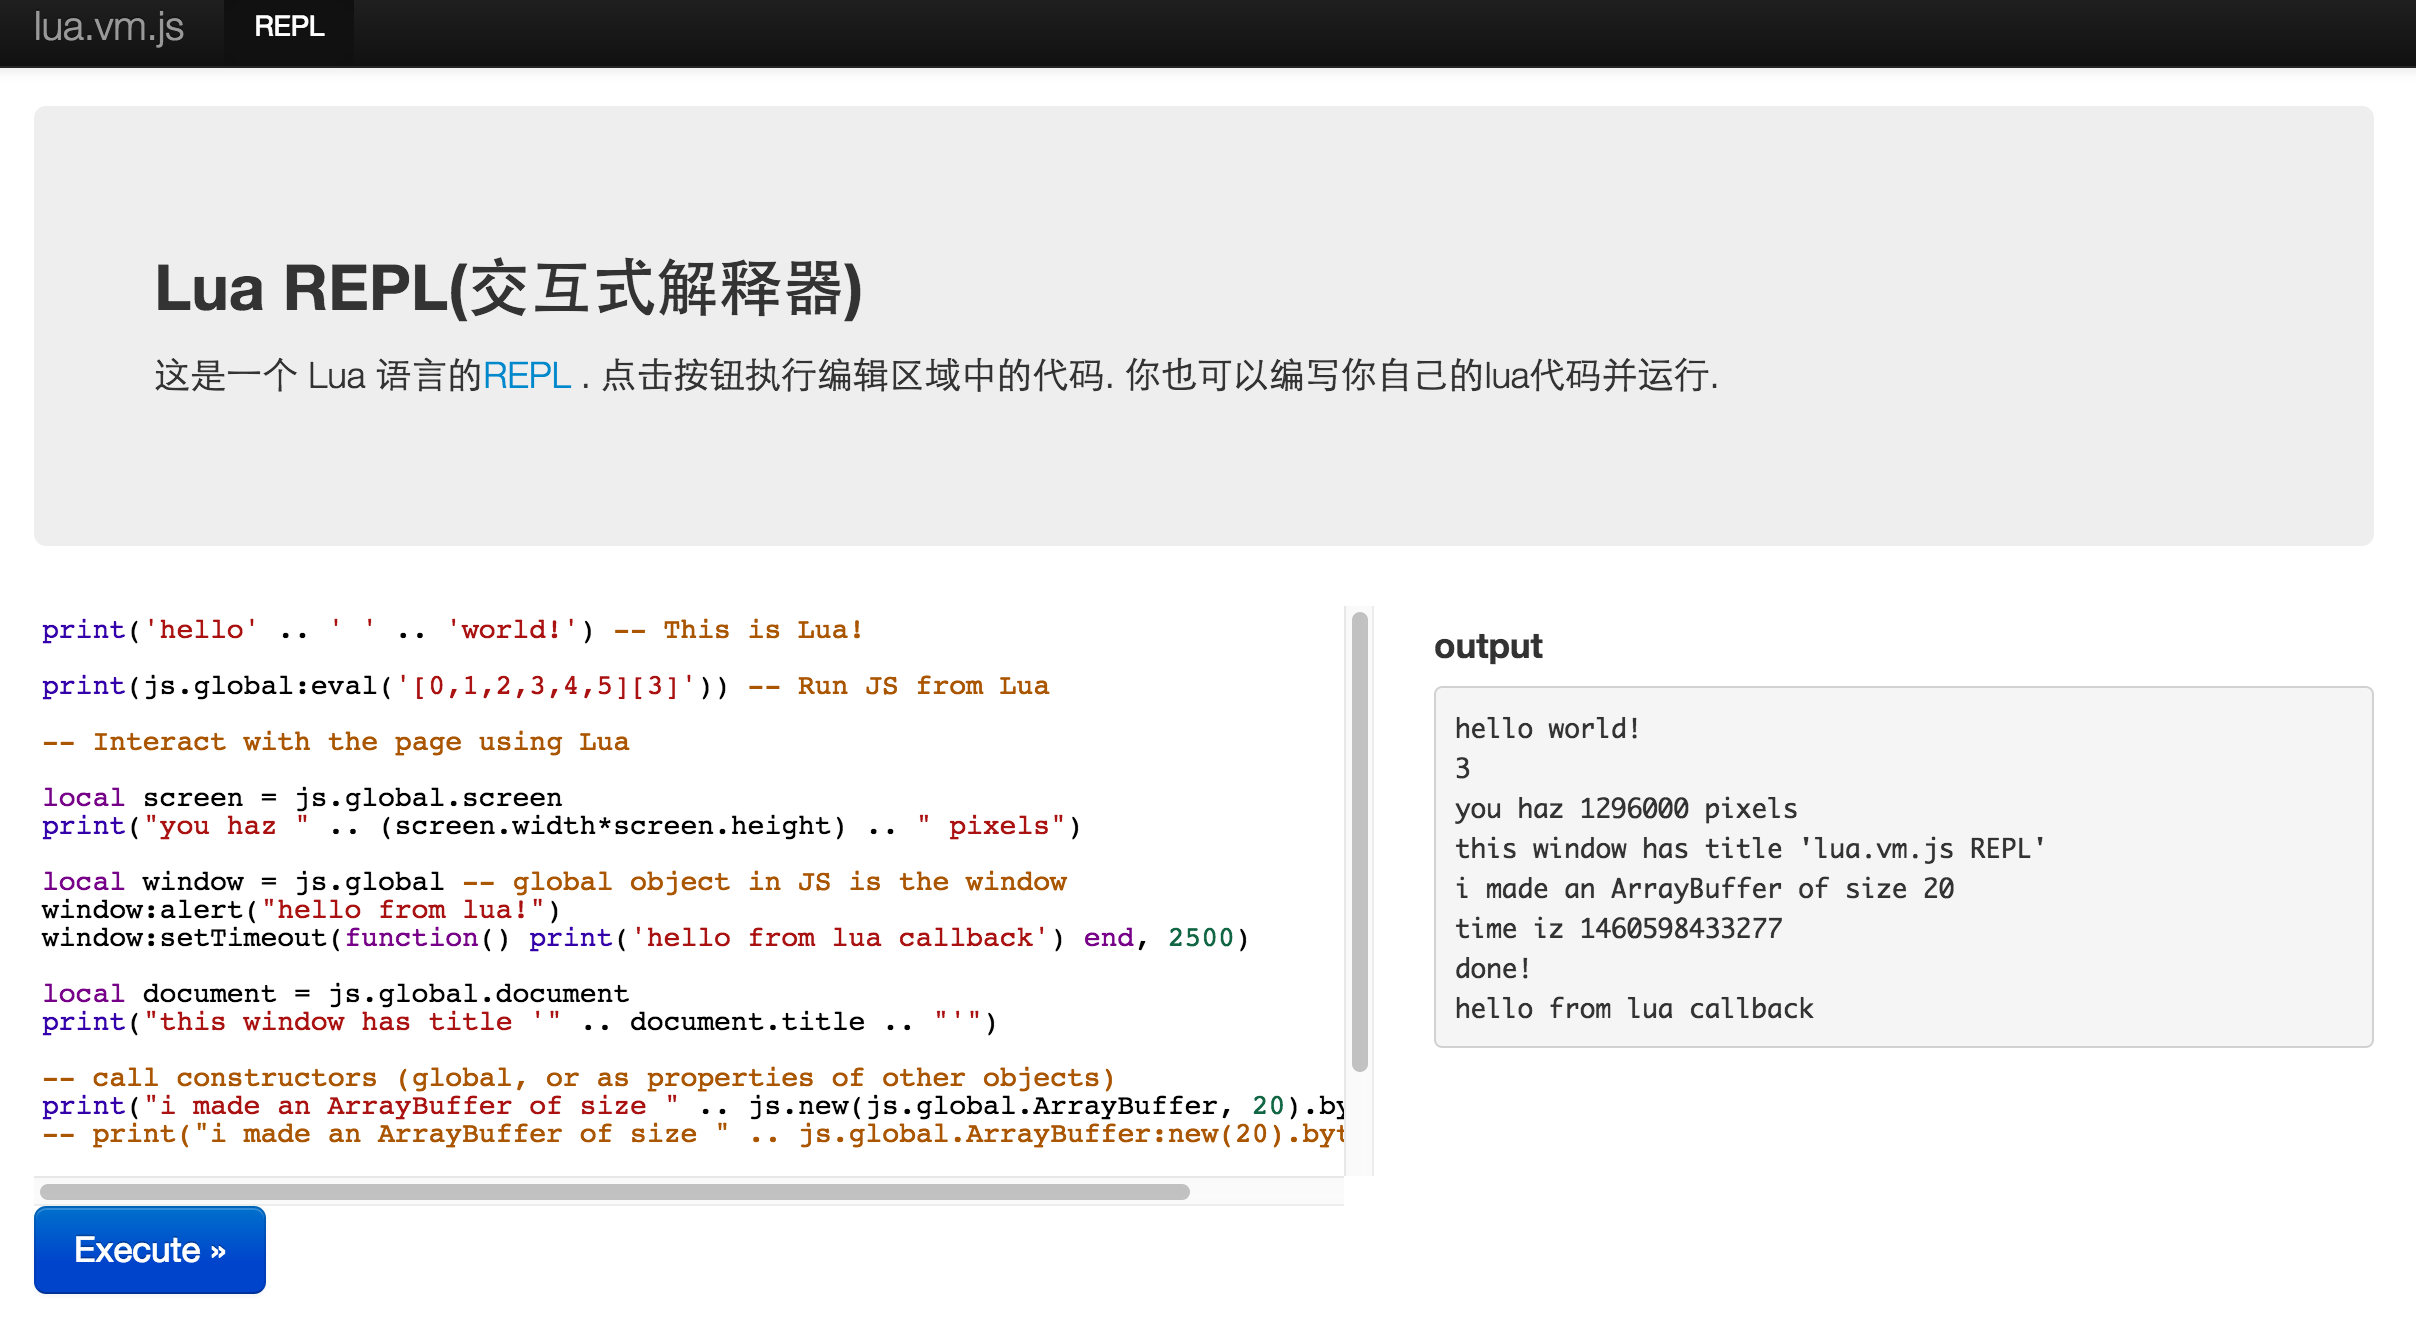
\includegraphics[width=400bp]{figure/pic/lua-vm-repl.png}
    \caption{lua REPL在浏览器中运行效果}
    \label{lua-vm-repl}
\end{figure}

该Web的左侧是一个textarea,可以编写Lua代码,编写好自己的Lua代码之后,点击Execute按钮,可以让代码运行。右侧的文本区是用来显示Lua代码的输出,和命令行REPL的终端窗口作用相同。